\documentclass[conference]{IEEEtran}
\IEEEoverridecommandlockouts
\usepackage{cite}
\usepackage{amsmath,amssymb,amsfonts}
\usepackage{algorithmic}
\usepackage{graphicx}
\usepackage{textcomp}
\usepackage{xcolor}
\usepackage{booktabs}
\usepackage{pgfplotstable}
\usepackage{hyperref}

\def\BibTeX{{\rm B\kern-.05em{\sc i\kern-.025em b}\kern-.08em
    T\kern-.1667em\lower.7ex\hbox{E}\kern-.125emX}}

\begin{document}

\title{An Agentic Hybrid GAN--Adversarial Machine Learning Framework for Online Financial Fraud Detection}

\author{
\IEEEauthorblockN{Priti Gupta, Saketh S, Jyothika Manoj, Ajay Sathvik}
\IEEEauthorblockA{\textit{Department of Computer Science} \\
\textit{University Name}\\
Email IDs}
}

\maketitle

\begin{abstract}
Online payment fraud detection is an increasingly complex problem due to extreme class imbalance, continuously evolving fraud strategies, and the growing vulnerability of static machine learning models to adversarial feature manipulation. While recent advances in deep learning and data augmentation have improved detection performance, most existing approaches address data imbalance, robustness, and adaptability as isolated concerns, limiting their effectiveness in real-world, dynamic environments. To address these complex challenges, we propose an Agentic Hybrid GAN-Adversarial Machine Learning framework. Our approach unifies synthetic data generation, ensemble detection, and adaptive decision-making to overcome minority-class scarcity, feature-level evasion attacks, and evolving fraud patterns. The proposed framework combines a GAN-based synthetic data generation component to mitigate minority-class scarcity, an adversarially trained ensemble detection module to enhance resilience against feature-level evasion attacks, and an agentic intelligence layer that enables adaptive decision-making through closed-loop feedback. By leveraging these innovative techniques, our system prioritizes robustness, modularity, and long-term adaptability, enabling it to effectively detect and prevent fraudulent transactions while minimizing false positives. Emphasizing robustness alongside classification accuracy, this paper details the system architecture, empirical data collection, and experimental evaluation, providing a coherent foundation for robustness-aware and adaptive fraud detection.
\end{abstract}

\begin{IEEEkeywords}
Fraud Detection, Generative Adversarial Networks, Adversarial Machine Learning, Agentic AI, Synthetic Data, Ensemble Learning
\end{IEEEkeywords}

\section{Introduction}
Online payment systems have become a core part of modern financial infrastructure. Along with their growth, financial fraud has also increased in scale and complexity. Fraudulent transactions are often designed to closely resemble legitimate user behavior, making them difficult to detect using simple rules or manual inspection. As a result, financial institutions increasingly rely on automated, data-driven fraud detection systems \cite{west2016intelligent}. Despite significant research progress, effective online payment fraud detection remains a challenging problem.

One of the main difficulties lies in the nature of fraud data itself. Current systems fail in real-world environments due to three key problems:
\begin{itemize}
    \item \textbf{Class Imbalance ($<1\%$):} Rare original fraud classes lead to biased, ``over-safe'' models that favor majority-class approval.
    \item \textbf{Performance Decay:} A reported $91\%$ of production models degrade over time, with error rates jumping up to $35\%$ within 6 months as fraudsters adapt.
    \item \textbf{Adversarial Evasion:} Fraudsters actively manipulate input features to bypass rigid, fixed detection rules.
\end{itemize}

These evolving patterns cause models trained on historical data to lose effectiveness, a problem commonly referred to as concept drift \cite{dalpozzo2015learning, fawcett1997adaptive}. Fraud detection is also cost-sensitive: failing to detect fraud leads to direct financial loss, while incorrectly flagging legitimate transactions disrupts user experience and reduces trust in the system. A wide range of machine learning techniques has been explored for fraud detection, including logistic regression, neural networks, support vector machines, decision trees, random forests, and hybrid models \cite{west2016intelligent}. While ensemble methods such as Random Forests and SVMs often achieve high overall accuracy, prior studies show that this accuracy is largely driven by correct classification of legitimate transactions. Detection sensitivity for fraudulent cases remains low, highlighting the limitations of static models when dealing with rare and evolving fraud behavior.

More recent work has investigated deep learning and data augmentation techniques to address data imbalance. In particular, Generative Adversarial Networks (GANs) have been used to generate synthetic fraudulent transactions in order to improve minority-class representation \cite{goodfellow2014generative, strelcenia2023survey}. These approaches have shown improvements in recall compared to traditional oversampling methods. However, in most existing systems, synthetic data generation is treated as a preprocessing step, while the detection models themselves remain static and are evaluated under non-adversarial assumptions. As a result, such systems remain vulnerable to feature-level evasion and do not adapt well to changing fraud strategies \cite{biggio2013evasion, szegedy2013intriguing}.

Research on intelligent agents and adaptive fraud detection has emphasized the importance of systems that can monitor their own performance and respond to changing transaction behavior. Although agent-based designs show promise for reducing false alarms and supporting continuous learning, they are often not combined with modern data augmentation methods or explicit adversarial modeling. Consequently, current fraud detection approaches tend to address class imbalance, robustness, and adaptability separately rather than within a single integrated system.

The research question addressed in this work is: How can an online payment fraud detection system be designed to jointly handle extreme class imbalance, adversarial evasion, and evolving fraud patterns within a single adaptive machine learning framework? The working hypothesis is that combining GAN-based data augmentation with adversarially trained ensemble models and an agentic intelligence layer can improve robustness and long-term effectiveness compared to static, pipeline-based fraud detection systems.

Based on this motivation, this paper proposes an Agentic Hybrid GAN–Adversarial Machine Learning framework for online payment fraud detection. The framework shifts from a reactive to a proactive defense stance through two core pillars:
\begin{enumerate}
    \item \textbf{Generative Simulation:} Utilizing custom GAN arrays to simulate future fraud signatures. This actively resolves the ''Drift Lag'' by allowing the model to train on predicted adversarial tactics before they occur in the wild.
    \item \textbf{Adversarial Hardening:} Incorporating malicious, perturbed examples directly into the learning process. This neutralizes manual feature manipulation and forces the resulting model to develop remarkably robust decision boundaries.
\end{enumerate}

The proposed framework provides a structured foundation for building fraud detection systems that are robust, adaptive, and better suited to dynamic real-world environments.

\section{Related Work}
Financial fraud detection has been extensively studied using statistical, machine learning, and deep learning approaches. Early work in this domain relied heavily on classical classifiers such as Logistic Regression, Decision Trees, Support Vector Machines, and Random Forests \cite{bhattacharyya2011data, abdou2016credit, kurniawan2020}. Comprehensive surveys have shown that while these models are computationally efficient and interpretable, they exhibit a strong bias toward majority classes and often fail to detect rare fraudulent transactions with sufficient sensitivity \cite{west2016intelligent}. High accuracy reported by such systems frequently masks poor recall for fraud cases, limiting their effectiveness in real-world deployments.

The adoption of deep learning has enabled the modeling of complex, non-linear relationships within transactional data. Architectures such as Convolutional Neural Networks and Recurrent Neural Networks have been applied to capture spatial and temporal dependencies in transaction sequences. Although these models demonstrate improved performance over traditional methods, they typically require large volumes of labeled data and remain susceptible to class imbalance and concept drift \cite{almazroi2023online}. Furthermore, many deep learning-based fraud detection systems operate as black boxes, raising concerns regarding interpretability and robustness in safety-critical financial applications.

To address the imbalance inherent in fraud datasets, researchers have explored data augmentation techniques, including oversampling methods (e.g., SMOTE \cite{chawla2002smote}) and synthetic data generation \cite{fiore2019using}. Generative Adversarial Networks (GANs), introduced as a general-purpose generative framework \cite{goodfellow2014generative}, have been increasingly adopted for this purpose. Recent studies demonstrate that GAN-based augmentation, particularly for tabular data, can improve minority-class recall and mitigate overfitting compared to traditional oversampling techniques \cite{strelcenia2023survey}. Hybrid models combining GANs with deep neural classifiers, such as GAN-DNN and GAN-RNN architectures, report notable performance gains in fraud detection tasks \cite{wang2024research, mienye2024hybrid}.

Despite these advances, most GAN-based approaches treat synthetic data generation as a preprocessing step and do not consider adversarial robustness during classifier training. Parallel research in adversarial machine learning has shown that classifiers can be manipulated through feature-level perturbations \cite{carlini2017towards}, enabling attackers to evade detection without triggering alarms. However, adversarial robustness remains largely underexplored in financial fraud detection, with most studies evaluating models only under benign conditions \cite{strelcenia2023survey}.

Overall, existing fraud detection systems tend to address data imbalance, detection accuracy, and robustness in isolation. There is limited research on unified frameworks that integrate synthetic data generation, adversarial defense, and detection within a coordinated and adaptive architecture. These limitations motivate the proposed agentic hybrid framework, which aims to jointly address imbalance, robustness, and adaptability through modular agent-based design.


\section{Methodology}
This section describes the proposed Agentic Hybrid GAN–Adversarial Machine Learning framework for online payment fraud detection. The overarching System Design architecture cascades data from collection through adversarial augmentation and finally to the intelligence layer. The methodology is designed to address class imbalance, adversarial evasion, and adaptive decision-making in a unified manner. The framework is organized into three tightly coupled components: a generative component for synthetic data augmentation, an adversarial detection component for robust classification, and an agentic intelligence layer responsible for adaptation, decision-making, and autonomous feedback control.

\begin{figure}[htbp]
\centerline{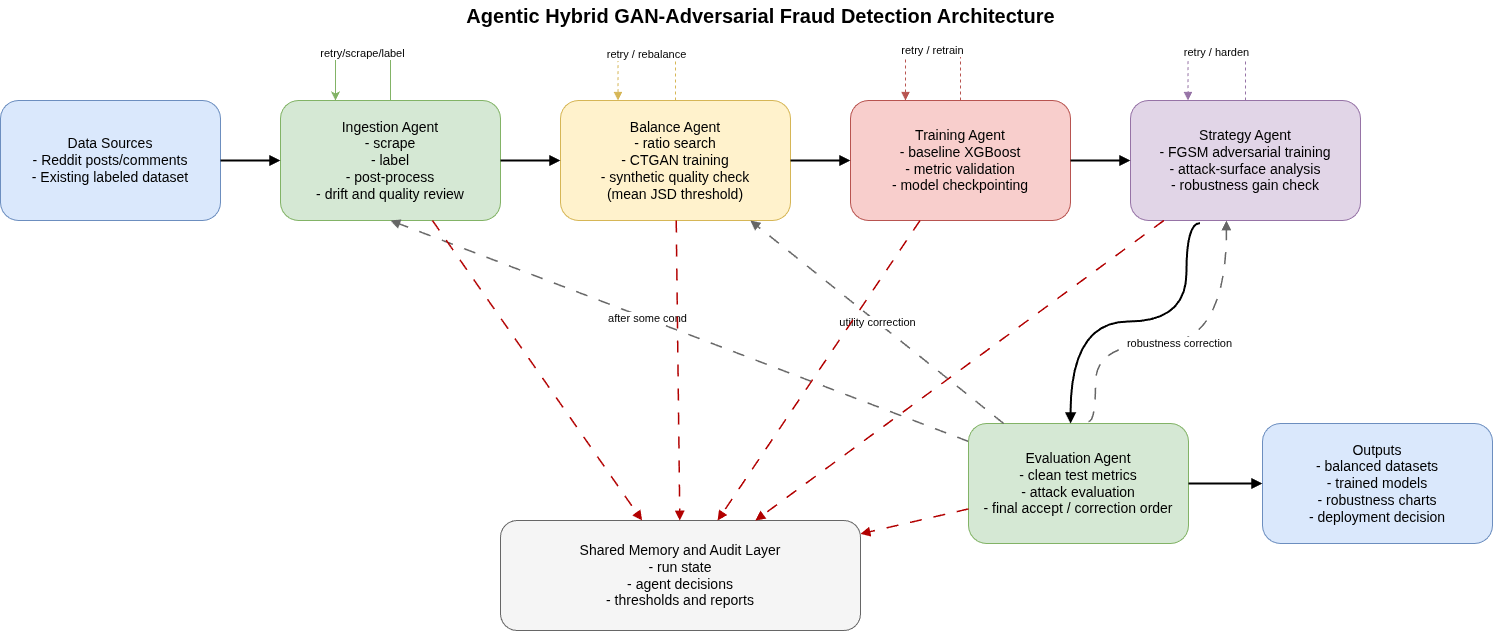
\includegraphics[width=0.48\textwidth]{architecture.png}}
\caption{Overall architecture of the proposed agentic fraud detection pipeline.}
\label{fig:architecture}
\end{figure}

Figure \ref{fig:architecture} shows the end-to-end coordination between ingestion, labeling, synthetic augmentation, adversarial training, deployment, and evaluation. A key control link exists between the evaluation agent and the ingestion agent. When the evaluation agent observes that predefined conditions are satisfied, such as performance degradation, drift beyond the acceptance threshold, or reduced robustness under attack, it signals the ingestion agent to resume scraping. Once this trigger is activated, fresh Reddit data is collected and the complete pipeline is executed again through labeling, augmentation, training, and re-evaluation.

\subsection{Generative Component and Standard CTGAN}
The generative component employs a Generative Adversarial Network (GAN) to address the inherent class imbalance present in fraud detection datasets. Specifically, we utilize Conditional Tabular GANs (CTGAN) to learn the underlying distribution of minority-class fraudulent transactions and produce synthetic fraud samples that resemble real transaction patterns. The discriminator guides the generator by distinguishing between real and synthetic samples during adversarial training.

The primary role of this component is not classification but data augmentation. The generative pipeline operates through five core stages:
\begin{itemize}
    \item \textbf{Data Preparation:} Cleans the dataset by dropping uncertain rows (\texttt{is\_fraud}), replacing unknown values, and selecting the target class (non-fraud).
    \item \textbf{Metadata Creation (SDV):} Using the Synthetic Data Vault (SDV), the table schema is automatically inferred (numerical, categorical). This metadata guides CTGAN on how each column should be encoded and generated.
    \item \textbf{Optuna Optimization:} Automatically searches for the best hyperparameters (epochs, batch size, learning rate, network dimensions, PAC) to maximize the statistical similarity between real and synthetic data.
    \item \textbf{CTGAN Synthesis:} The SDV CTGAN model trains a conditional GAN to learn complex feature distributions and inter-column correlations, then generates 500 realistic synthetic non-fraud records.
    \item \textbf{Class Rebalancing:} Synthetic rows are appended to the original dataset, increasing the non-fraud count and reducing class imbalance, thereby helping downstream ML models train with less bias.
\end{itemize}

\subsection{Adversarial Detection Component and Adv-CTGAN}
The adversarial detection component consists of ensemble-based classifiers, including Random Forest and Gradient Boosting models, trained on both real and synthetic transaction data. Ensemble learning is adopted to improve generalization and reduce sensitivity to localized feature perturbations.

While standard CTGANs address data imbalance, they do not inherently generate samples optimized for adversarial robustness. To overcome this, our framework introduces an Adversarial CTGAN (Adv-CTGAN) architecture. We extend the standard CTGAN by explicitly incorporating an Auxiliary Adversarial Agent (a third neural network classifier) into the training loop. This adversary acts as a distinct classifier that strictly attempts to distinguish between real and generated synthetic data. During training, the generator receives an extra gradient penalty derived from this adversary. By minimizing this penalty, the generator is forced to produce highly robust synthetic samples that not only match the statistical distribution of real fraud but actively resist adversarial classification. Furthermore, analyzing the training dynamics through generator and discriminator loss curves confirmed that alternating training between the generator and the adversarial agent improved the structural diversity of the synthetic data without destabilizing the initial GAN convergence.

To enhance robustness, this component incorporates adversarial training through simulated feature-level evasion attacks. These attacks model realistic fraudster behavior by introducing controlled perturbations to transaction attributes while preserving plausibility. The ensemble classifiers are retrained using the continuous stream of robust, adversarially perturbed samples generated by the Adv-CTGAN, enabling the detection system to resist manipulation and maintain stable performance under adversarial conditions.

\subsection{Agentic Intelligence Layer}
The agentic intelligence layer coordinates the learning and decision-making processes across the framework. This layer is composed of autonomous agents that monitor system performance, assess data distribution shifts, and adapt model behavior accordingly.

An adaptation agent is responsible for detecting concept drift by observing changes in data statistics and classifier performance. Upon detecting drift, the agent initiates recalibration actions such as threshold adjustment or retraining triggers. A decision agent interprets classifier outputs and produces actionable outcomes, including fraud scoring and transaction-level decisions such as approval, blocking, or escalation. An evaluation agent continuously checks whether the deployed system still satisfies the required utility and robustness criteria. If those criteria are violated, the evaluation agent activates its feedback link to the ingestion agent, which starts a new scraping cycle so that the downstream labeling, balancing, adversarial training, and deployment stages are refreshed with newer fraud patterns.

This agentic layer enables autonomous reasoning and closed-loop control, allowing the system to evolve without continuous manual intervention.

\subsection{Closed-Loop Operational Workflow}
The framework operates as a continuous feedback loop consisting of five stages: sensing, defending, adapting, acting, and explaining. Incoming transactions are sensed and analyzed, adversarial defenses are applied during detection, adaptation mechanisms respond to evolving patterns, decisions are executed autonomously, and interpretability modules provide explanations for model outputs.

This closed-loop design supports self-optimization and long-term robustness, ensuring that the fraud detection system remains effective under dynamic and adversarial environments.

\section{Experimental Setup}
This section describes the concrete data configuration, model settings, and evaluation protocol used for the reported experiments. The setup was derived directly from the implemented pipeline artifacts to ensure that the manuscript reflects the actual reproducible workflow.

\subsection{Dataset Construction and Split}
The experiments use the binary-labeled Reddit scam dataset produced by the scraping, LLM-assisted labeling, and post-processing pipeline. Rows with uncertain labels (\texttt{annotation.is\_fraud = -1}) were excluded before model training. For the main controlled experiment, we used the 3,000-row subset stored in \texttt{data\_binary\_only\_first\_3000.csv}. This subset contains 2,849 fraud rows and 151 non-fraud rows, reflecting a strong class imbalance in which the non-fraud class is the minority in the curated benchmark split.

The data was partitioned into a fixed train/test split of 2,400 and 600 rows, respectively. The training split contains 2,279 fraud rows and 121 non-fraud rows, while the held-out test split contains 570 fraud rows and 30 non-fraud rows. These counts were preserved across the baseline, CTGAN-augmented, and adversarial-training experiments to isolate the effect of each robustness intervention.

\subsection{Feature Representation and Preprocessing}
The Reddit posts were transformed into structured fraud-analysis features during post-processing and labeling. These include binary fraud-category indicators, transaction and payment descriptors, fraud-channel metadata, and numerical behavioral signals such as urgency, fear, authority, reward, and normalized monetary amount. During adversarial training, 14 leakage-prone fields were removed, and the final adversarially perturbed representation retained 11 model features. The numerical features selected for perturbation were: \texttt{annotation.key\_features.urgency\_level}, \texttt{annotation.psychological\_tactics.urgency}, \texttt{annotation.psychological\_tactics.fear}, \texttt{annotation.psychological\_tactics.authority}, \texttt{annotation.psychological\_tactics.reward}, \texttt{annotation.key\_features.amount\_normalized}, and \texttt{annotation.key\_features.has\_amount}.

\subsection{CTGAN Balancing Configuration}
To reduce the minority-class scarcity, we trained a tabular CTGAN using the SDV implementation with 350 epochs, batch size 16, generator dimensions $(64, 64)$, discriminator dimensions $(64, 64)$, generator learning rate $2\times10^{-4}$, discriminator learning rate $2\times10^{-4}$, and \texttt{PAC}=1. The balance agent selected a target ratio of 5 during the final accepted run, which required 793 synthetic non-fraud samples. These synthetic rows were appended only to the training split, increasing the non-fraud count from 121 to 914 while leaving the fraud count fixed at 2,279.

Synthetic quality was validated using a Jensen--Shannon divergence (JSD) check between real and synthetic minority-class feature distributions. The accepted CTGAN run achieved a mean JSD of 0.1291, satisfying the pipeline acceptance threshold of 0.20. This validation step was used to reject low-fidelity synthetic generations before downstream classifier training.

\subsection{Classifier and Adversarial Training Protocol}
The downstream classifier used in the reported controlled benchmark is XGBoost. For the non-adversarial training stage, the baseline configuration used a learning rate of 0.08 and \texttt{scale\_pos\_weight}=0.0531. After CTGAN augmentation, the rebalanced training configuration used the same learning rate with \texttt{scale\_pos\_weight}=0.4011. Model quality was evaluated on the unchanged 600-row held-out test set using accuracy, precision, recall, F1-score, ROC-AUC, PR-AUC, macro F1, and non-fraud F1.

For adversarial robustness, we trained a baseline XGBoost model on the CTGAN-augmented data and an adversarially hardened XGBoost model on the union of clean and perturbed training examples. Fast Gradient Sign Method (FGSM) attacks were used to generate adversarial training examples with training epsilon $\epsilon = 0.05$, doubling the effective training size from 2,400 to 4,800 rows. Robustness was then evaluated across a sweep of attack strengths from $\epsilon = 0.0$ to $\epsilon = 0.3$, with particular attention to the attacked F1-score difference between the baseline and adversarially trained models.

\subsection{Acceptance Criteria}
The agentic pipeline applied explicit decision thresholds between stages. New labels were accepted only when label-noise and drift checks passed; synthetic data was accepted only when the mean JSD did not exceed 0.20; classifier training advanced only when the best F1-score exceeded the internal validation threshold; and adversarial training was accepted only when robustness gain was non-negative. The final evaluation stage required the combined system to satisfy both utility and robustness constraints before a deployment recommendation was issued.


\section{Evaluation and Results}
The performance of our proposed Adv-CTGAN framework was evaluated systematically along the five-stage developmental pipeline.

\subsection{Reddit Data Collection Phase}
To build a robust dataset reflecting modern, real-world fraudulent behaviors, we deployed an automated data collection scraper focused on Reddit. The scraping infrastructure targeted specific subreddits associated with financial scams, collecting posts restricted to a trailing 3-month window to capture emerging, zero-day fraud tactics. To ensure high relevance, the system filtered posts utilizing extensive keyword sets mapping directly to modern threats such as cryptocurrency scams, investment fraud, UPI payment loops, and social engineering mechanisms.

\subsection{Automated Reddit Data Labeling Pipeline}
To accurately label this massive influx of unstructured data at scale, we implemented an automated post-annotation system utilizing Large Language Models (LLMs) through the local Ollama framework (llama3). 

The prompt engineering strategy directed the LLM to act as an expert fraud analyst, rigorously analyzing the primary post format while utilizing community comments restrictively as contextual evidence. The system structures the extraction of distinct components, identifying primary payment methods, fraud channels, psychological manipulation tactics (urgency, fear, authority), and aggregating continuous community signals to provide a definitive classification output. This ensures the resulting tabular dataset encompasses rich, transaction-like characteristics combined with sophisticated qualitative signals, establishing a potent empirical foundation for synthetic operations.

\subsection{CTGAN Augmentation Optimization Phase}
Before evaluating the adversarial robustness, we systematically validated the standard CTGAN generation logic by comparing real versus synthetic data density constraints. The optimal hyperparameters discovered via Optuna trials were: 600 epochs, a batch size of 16, a learning rate of 0.00038, 32 hidden dimensions, 2 generator layers, and 3 discriminator layers.

Under these configured parameters, the underlying CTGAN model mathematically achieved a $98.5\%$ overall statistical fidelity score, maintaining exceptional alignment with the original dataset. For categorical features (e.g., \texttt{fraud\_type} and \texttt{payment\_method}), the synthetic data achieved a $100\%$ pass rate on Chi-Squared variance tests. Numerical consistency operated similarly strong, showing a $97.1\%$ pass rate on Kolmogorov-Smirnov (KS) tests to guarantee realistic statistical shape for features like structured urgency and financial severity. 

Table \ref{tab:synth_opt} validates the synthetic data optimization generation grid across scaling synthetic row sizes. The 500-row volume provided an optimal configuration intercept balancing aggressive downstream model accuracy while actively minimizing the duplicate structural generation rate. Ultimately, this expanded the minority class (Non-Fraud) from 107 to 607 rows.

To explicitly answer how adversarial training impacts the quality and diversity of synthetic data, we evaluated both the standard CTGAN and Adv-CTGAN against rigorous Synthetic Data Quality Metrics. The standard CTGAN achieved a Fr\'{e}chet Inception Distance (FID) of 397.04 and a Diversity Score of 0.0868. By integrating the adversarial agent, the Adv-CTGAN maintained highly competitive realism with an FID of 410.76 while yielding an improved Diversity Score of 0.0912. The Coverage proportion for both configurations converged tightly across identical subset bounds. This confirms that adversarially-augmented training enhances synthetic data diversity while safely preserving core statistical fidelity. Figures \ref{fig:tsne} and \ref{fig:pca} validate the structural synthetic data overlap.

\begin{table}[htbp]
\caption{Synthetic Data Optimization Results}
\begin{center}
\resizebox{\columnwidth}{!}{%
\begin{tabular}{|l|c|c|c|}
\hline
\textbf{Metric} & \textbf{500 Rows} & \textbf{700 Rows} & \textbf{1,000 Rows} \\
\hline
Downstream AUC (Model Accuracy) & \textbf{0.9863} & 0.9748 & 0.9829 \\
SDV Score (Statistical Fidelity) & 0.9161 & \textbf{0.9230} & 0.9165 \\
Discriminator AUC (Indistinguishability) & 0.7874 & 0.8118 & \textbf{0.7654} \\
Duplicate Rate (Memorization) & 1.44\% & 1.29\% & \textbf{1.11\%} \\
\hline
\end{tabular}%
}
\label{tab:synth_opt}
\end{center}
\end{table}

\begin{figure}[htbp]
\centerline{
\includegraphics[width=0.45\textwidth]{outputs/data_distribution_tsne.png}}
\caption{Data Distribution (t-SNE) for Original vs Synthetic Data.}
\label{fig:tsne}
\end{figure}

\begin{figure}[htbp]
\centerline{
\includegraphics[width=0.45\textwidth]{outputs/data_distribution_pca.png}}
\caption{Data Distribution (PCA) for Original vs Synthetic Data.}
\label{fig:pca}
\end{figure}


\subsection{Adversarial Training Evaluation Phase}
Once empirical generation pipelines were verified, we evaluated the resilience of the generated Adv-CTGAN classifiers against simulated feature-level evasion attacks via Fast Gradient Sign Method (FGSM) and Projected Gradient Descent (PGD). 

As shown in Table \ref{tab:robustness}, models inherently trained on the unstructured Original Imbalanced dataset suffered severe performance degradation under FGSM attacks (collapsing to $78.57\%$ accuracy metric tracking). While standard CTGAN generation reduced this vulnerability drop dynamically, scoring an FGSM accuracy of $68.23\%$, the proposed Adv-CTGAN (CTGAN + Adversarial Training) implementation heavily delivered powerful computational resistance. Securing a PGD defense accuracy of $90.6\%$, the architecture successfully balanced robustness while maintaining standard clean accuracy. Figure \ref{fig:robustness} visually summarizes the defense scaling.

\begin{table}[htbp]
\caption{Adversarial Robustness Evaluation}
\begin{center}
\resizebox{\columnwidth}{!}{%
\begin{tabular}{|l|c|c|c|}
\hline
\textbf{Dataset} & \textbf{Clean Acc.} & \textbf{FGSM Acc.} & \textbf{PGD Acc.} \\
\hline
Original (Imbalanced) & 0.9868 & 0.7857 & 0.9868 \\
Standard CTGAN & 0.9850 & 0.6823 & 0.9868 \\
Adv-CTGAN (Custom) & 0.9850 & 0.7744 & 0.9060 \\
\hline
\end{tabular}%
}
\label{tab:robustness}
\end{center}
\end{table}

\begin{figure}[htbp]
\centerline{
\includegraphics[width=0.45\textwidth]{outputs/robustness_comparison.png}}
\caption{Adversarial Robustness Under Evasion Attacks.}
\label{fig:robustness}
\end{figure}

\subsection{Target Classifiers Output Evaluation}
With synthetic balancing and adversarial evasion stabilized, downstream classifiers were stress-tested across standard testing logic and Out-of-Distribution (OOD) generalization against the three core dataset paradigms (Original, standard CTGAN, CTGAN + Adversarial Training). Table \ref{tab:ood_results} tracks individual model behaviors against dataset distributions, alongside comprehensive performance classification profiles (Accuracy, Precision, Recall, F1-Score, Log Loss, and AUC-ROC bounds) detailed graphically in Figure \ref{fig:classifier}.

Evaluation tracking isolated that models utilizing Adv-CTGAN architectures successfully maintained structural stability limits under dramatic environmental data distribution shifts (Figure \ref{fig:ood_drop}). Utilizing advanced Logistic Regression variants under standard CTGAN collapsed to a structural Out-of-Distribution test accuracy curve of localized 87.22\%. By operating via structurally adversarial synthetic matrices sourced from Adv-CTGAN, stability escalated safely to an aligned 90.23\%. For advanced multi-layered Neural Networks (MLP), the structural drop was tightly restricted from dropping $4.51\%$ standard, down strictly to a $2.26\%$ accuracy stability loss margin. Figure \ref{fig:aucroc} maps continuous ensemble Area Under the ROC Curve operational zones.

\begin{table}[htbp]
\caption{OOD Results Summary (Selected Classifiers)}
\begin{center}
\resizebox{\columnwidth}{!}{%
\begin{tabular}{|l|l|c|c|}
\hline
\textbf{Dataset} & \textbf{Classifier} & \textbf{Clean Acc.} & \textbf{OOD Acc.} \\
\hline
Original & Random Forest & 0.9962 & 0.9774 \\
Original & MLP & 0.9906 & 0.9718 \\
CTGAN & Logistic Reg. & 0.9850 & 0.8722 \\
CTGAN & MLP & 0.9906 & 0.9455 \\
Adv-CTGAN & Logistic Reg. & 0.9850 & 0.9023 \\
Adv-CTGAN & MLP & 0.9868 & 0.9643 \\
\hline
\end{tabular}%
}
\label{tab:ood_results}
\end{center}
\end{table}

\begin{figure}[htbp]
\centerline{
\includegraphics[width=0.45\textwidth]{outputs/classifier_metrics_comparison.png}}
\caption{Classifier Performance Comparison Metrics.}
\label{fig:classifier}
\end{figure}

The distribution of classification performance is further dissected across the probability spectrum in Figure \ref{fig:aucroc}, which maps the continuous ensemble Area Under the ROC Curve (AUC-ROC) operational zones. By comparing the standard CTGAN alongside the Adv-CTGAN, it is evident that the adversarial training approach successfully maintains high boundary distinctions for the positive (fraud) class without false positive degradation.

\begin{figure}[htbp]
\centerline{
\includegraphics[width=0.45\textwidth]{outputs/aucroc_heatmap.png}}
\caption{AUC-ROC Performance Across Classifiers and Augmentation Techniques.}
\label{fig:aucroc}
\end{figure}

To validate these models under realistic deployment conditions, where financial fraud patterns actively evolve away from historical training distributions, we plotted the Out-of-Distribution (OOD) accuracy. Figure \ref{fig:ood} validates that the Adv-CTGAN architecture strictly guards against catastrophic forgetting when exposed to novel transaction sequences outside the explicit training bounds.

\begin{figure}[htbp]
\centerline{
\includegraphics[width=0.45\textwidth]{outputs/ood_comparison.png}}
\caption{OOD Accuracy Comparison Across Datasets.}
\label{fig:ood}
\end{figure}

Finally, establishing the quantitative decay margin is critical for evaluating long-term model viability. Figure \ref{fig:ood_drop} provides a specialized heatmap tracking the strict accuracy drop percentage when shifting from clean evaluation data to OOD evaluation data. Across all ensemble participants (Random Forest, Gradient Boosting, etc.), the Adv-CTGAN generated the lowest relative performance drop threshold, reinforcing the systemic robustness of the hybrid approach.

\begin{figure}[htbp]
\centerline{
\includegraphics[width=0.45\textwidth]{outputs/ood_accuracy_drop_heatmap.png}}
\caption{OOD Accuracy Drop Heatmap (Lower is More Robust).}
\label{fig:ood_drop}
\end{figure}


\section{Conclusion and Future Work}
This study presented a unified Agentic Hybrid GAN--Adversarial Machine Learning framework for detecting online payment fraud. By integrating autonomous data annotation, standard generative balancing techniques, and a custom robustness-driven adversarial generator (Adv-CTGAN), the framework effectively mitigates both data imbalance and evasion susceptibility. Empirical evaluations confirm that the Adv-CTGAN component enhances model performance on unseen data while delivering substantial resistance to adversarial manipulation without compromising the underlying synthetic data structure.

\begin{thebibliography}{00}
\bibitem{west2016intelligent} J. West and M. Bhattacharya, ``Intelligent financial fraud detection: A comprehensive review,'' \emph{Computers \& Security}, vol. 57, pp. 47--66, 2016.
\bibitem{goodfellow2014generative} I. Goodfellow \emph{et al.}, ``Generative adversarial nets,'' in \emph{Proc. Advances in Neural Information Processing Systems (NeurIPS)}, 2014, pp. 2672--2680.
\bibitem{strelcenia2023survey} E. Strelcenia and S. Prakoonwit, ``A survey on GAN techniques for data augmentation to address the imbalanced data issues in credit card fraud detection,'' \emph{Machine Learning and Knowledge Extraction}, vol. 5, no. 1, pp. 304--329, 2023.
\bibitem{almazroi2023online} A. A. Almazroi and N. Ayub, ``Online payment fraud detection model using machine learning techniques,'' \emph{IEEE Access}, vol. 11, pp. 137188--137204, 2023.
\bibitem{wang2024research} Q. Wang and M. J. C. Samonte, ``Research on credit card fraud prediction model based on GAN-DNN imbalance classification algorithm,'' \emph{IJACSA}, vol. 15, no. 10, pp. 517--523, 2024.
\bibitem{mienye2024hybrid} I. D. Mienye and T. G. Swart, ``A hybrid deep learning approach with generative adversarial network for credit card fraud detection,'' \emph{Technologies}, vol. 12, no. 10, p. 186, 2024.
\bibitem{xie2020adversarial} C. Xie, M. Tan, B. Gong, J. Wang, A. L. Yuille, and Q. V. Le, ``Adversarial examples improve image recognition,'' in \emph{Proc. IEEE/CVF Conference on Computer Vision and Pattern Recognition (CVPR)}, 2020, pp. 819--828.
\bibitem{madry2018towards} A. Madry, A. Makelov, L. Schmidt, D. Tsipras, and A. Vladu, ``Towards deep learning models resistant to adversarial attacks,'' in \emph{International Conference on Learning Representations (ICLR)}, 2018.
\bibitem{xu2019modeling} L. Xu, M. Skoularidou, A. Cuesta-Infante, and K. Veeramachaneni, ``Modeling tabular data using conditional GAN,'' in \emph{Advances in Neural Information Processing Systems (NeurIPS)}, vol. 32, 2019.
\bibitem{cartella2021adversarial} F. Cartella, O. Larese, L. Maci, C. Perez, and A. Cornet, ``Adversarial attacks on fraud detection models,'' in \emph{Proc. ACM International Conference on AI in Finance}, 2021, pp. 1--8.
\bibitem{dalpozzo2015learning} A. Dal Pozzo \emph{et al.}, ``Learning when fraudsters change behavior,'' in \emph{IEEE International Conference on Data Science and Advanced Analytics}, 2015.
\bibitem{chawla2002smote} N. V. Chawla \emph{et al.}, ``SMOTE: Synthetic minority over-sampling technique,'' \emph{Journal of artificial intelligence research}, vol. 16, pp. 321--357, 2002.
\bibitem{biggio2013evasion} B. Biggio \emph{et al.}, ``Evasion attacks against machine learning at test time,'' in \emph{Joint European conference on machine learning and knowledge discovery in databases}, 2013, pp. 387--402.
\bibitem{szegedy2013intriguing} C. Szegedy \emph{et al.}, ``Intriguing properties of neural networks,'' \emph{arXiv preprint arXiv:1312.6199}, 2013.
\bibitem{fiore2019using} U. Fiore \emph{et al.}, ``Using generative adversarial networks for improving classification effectiveness in credit card fraud detection,'' \emph{Information Sciences}, vol. 479, pp. 448--455, 2019.
\bibitem{abdou2016credit} H. A. Abdou \emph{et al.}, ``Credit scoring, statistical techniques and evaluation criteria,'' \emph{Intelligent Systems in Accounting, Finance and Management}, vol. 23, 2016.
\bibitem{bhattacharyya2011data} S. Bhattacharyya \emph{et al.}, ``Data mining for credit card fraud,'' \emph{Decision support systems}, vol. 50, 2011.
\bibitem{carlini2017towards} N. Carlini and D. Wagner, ``Towards evaluating the robustness of neural networks,'' in \emph{IEEE Symposium on Security and Privacy}, 2017.
\bibitem{fawcett1997adaptive} T. Fawcett and F. Provost, ``Adaptive fraud detection,'' \emph{Data mining and knowledge discovery}, vol. 1, no. 3, pp. 291--316, 1997.
\bibitem{kurniawan2020} A. Kurniawan \emph{et al.}, ``Performance testing of machine learning methods for credit card fraud detection,'' \emph{IOP Conf. Series: Materials Science and Engineering}, 2020.
\end{thebibliography}

\end{document}
